\chapter{Late-Stage Stars and Disks}
\label{ch:late_disk}

\marginnote{
\textbf{Suggested background reading:}
\begin{itemize}
\item \href{http://adsabs.harvard.edu/abs/2014prpl.conf..475A}{Alexander, R., et al. 2014, in "Protostars and Planets VI", ed.~H.~Beuther et al., pp.~475-496} \nocite{alexander14a}
\end{itemize}
\textbf{Suggested literature:}
\begin{itemize}
\item \href{http://adsabs.harvard.edu/abs/2001ApJ...560..957D}{Dullemond, C.~P., Dominik, C., \& Natta, A. 2001, ApJ, 560, 957} \nocite{dullemond01a}
\item \href{http://adsabs.harvard.edu/abs/2009ApJ...700.1502A}{Andres, S.~M., et al. 2009, ApJ, 700, 1502} \nocite{andrews09a}
\end{itemize}
}

The last two chapters of this book are concerned with the fate of the left-over material from the star formation process, which is mostly collected into accretion disks around them. This chapter discusses how this material is dispersed, and the final one introduces the process by which it can begin to form planets.

\section{Stars Near the End of Star Formation}

We will begin our study of the final stages of star formation with a discussion of the stars themselves. The stars we want to study are ones that fall into the class II and class III category, and are observationally classified as either T Tauri or Herbig Ae/Be stars.\footnote{Roughly speaking, T Tauri stars are objects below $\sim 2$ $\msun$, of spectral type G0 or later, and Herbig Ae/Be stars are more massive objects of earlier spectral types. While the spectra of these two types of objects are different due to their differing surface temperatures, they appears to share a common physical nature and evolutionary history. Consequently we will discuss them as a single class in this chapter.} These stars no longer have envelopes of material around them that are sufficient to obscure the stellar photosphere. However, they are young enough that they still exhibit various signs of youth. The presence of a disk is one of these signs.

\subsection{Optical Properties}

The main observational signature that has been used historically to define the T Tauri and Herbig Ae/Be classes is the presence of excess optical spectral line emission beyond that expected for a main sequence star of the same spectral class. The most prominent such line is H$\alpha$, the $n=3\rightarrow 2$ line for hydrogen, along with other hydrogen Balmer lines (Figure \ref{fig:tts_appenzeller89}). H$\alpha$ is particularly striking because in almost all main sequence objects H$\alpha$ is seen in absorption rather than emission. The strength of the H$\alpha$ emission in T Tauri stars ranges from equivalent widths (EW) of $\sim 100$ \AA\ down to zero -- which still makes the stars stand out from main sequence stars, which have H$\alpha$ absorption. We divide T Tauri stars into classical ones, defined as those with H$\alpha$ EW $\gtrsim 10$ \AA, and weak-lined, those with H$\alpha$ EW $\lesssim 10$ \AA. Both classes also often show variability in their H$\alpha$ line profiles on periods of hours or days.

A large number of other optical and UV emission lines are also seen from these stars, and their strength generally correlates with that of the H$\alpha$ line. In addition to optical and ultraviolet line emission, these stars also exhibit the property of continuum veiling. What this means is that, in addition to excess line emission, these stars show excess continuum emission beyond what would be expected for a bare stellar photosphere. This excess emission arises from above the photospheric region where absorption occurs, so these photons are not absorbed. As a result they can partially or completely fill in normal photospheric absorption lines, reducing their equivalent width -- hence the name veiling.

\begin{marginfigure}
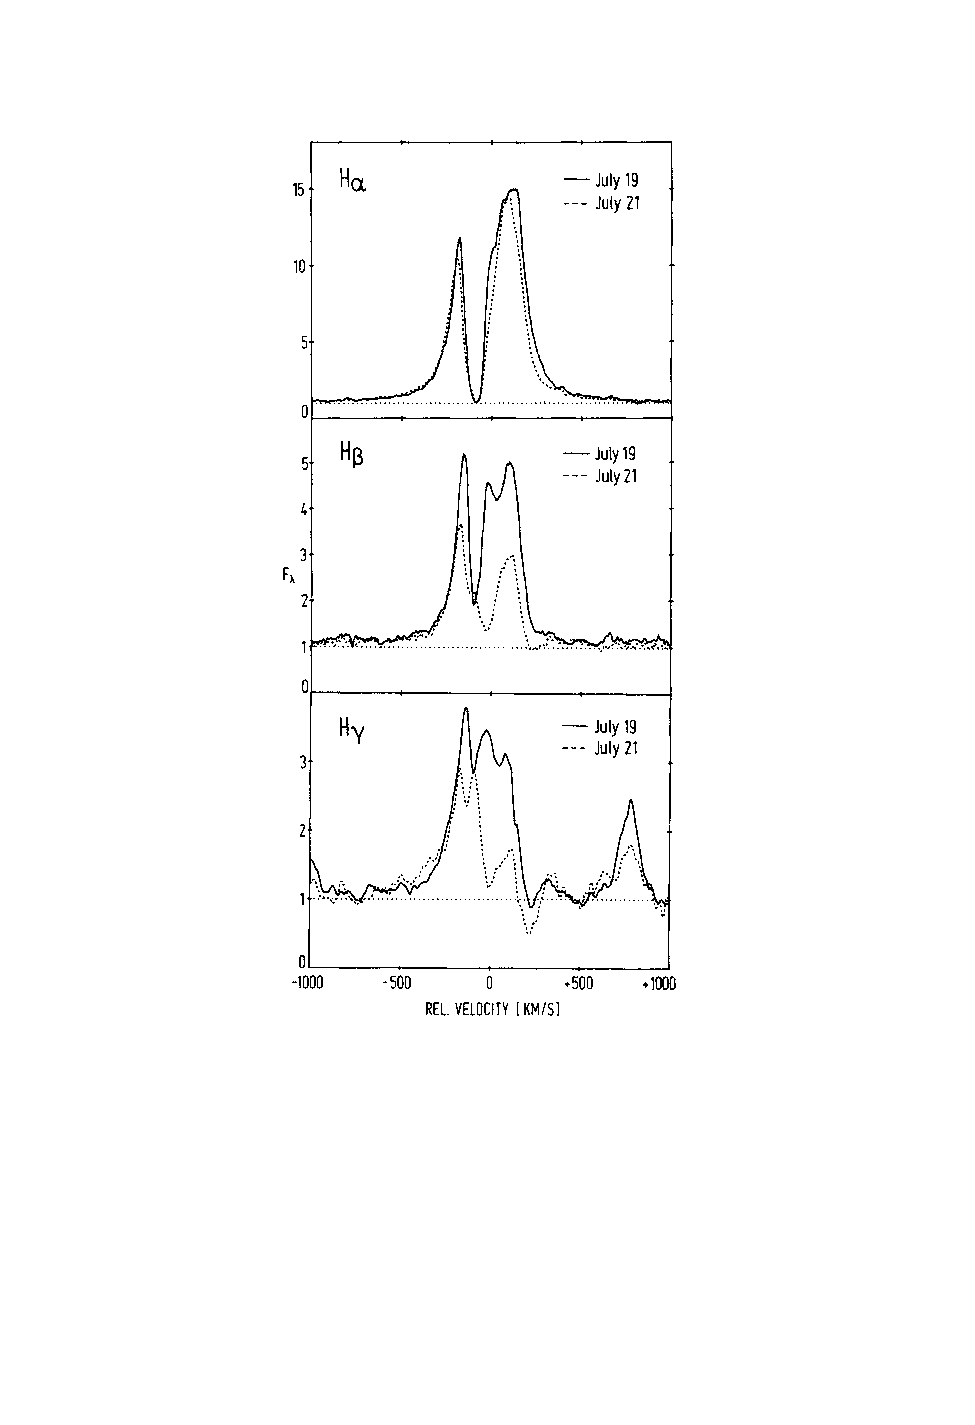
\includegraphics[width=\linewidth]{tts_appenzeller89}
\caption[Balmer lines of T Tauri stars]{
\label{fig:tts_appenzeller89}
Observed line profiles for three Balmer lines from the T Tauri star S Cr A taken on two nights in July, 1983. Credit: Astron.~\& Astrophys.~Rev., ``T Tauri Stars", 1, 1989, 291, \citeauthor{appenzeller89a}. With permission of Springer.
}
\end{marginfigure}

\subsection{Infall Signatures}

The H$\alpha$ is particularly interesting, because it tells us something about the star's immediate environment. For main sequence stars, the H$\alpha$ line profile is a result of absorption at the stellar photosphere and emission from the chromosphere. At the photosphere there is a population of neutral hydrogen atoms in the $n=2$ level that absorbs photons at H$\alpha$ frequencies, producing absorption. Above that in the chromosphere is an optically thin, hot gas, which contains atoms in the $n=3$ level. Some of these emit H$\alpha$ photons, partially filling in the absorption trough, but leaving the line overall in absorption.

Producing H$\alpha$ in emission is tricky, however. The emitting material must be above the stellar photosphere, so it can fill in the absorption trough created there. This gas must be at temperatures of $5,000-10,000$ K to significantly populate the $n=3$ level. However, in order to produce enough H$\alpha$ photons to fill in the trough and produce net emission, this gas must also be dense enough for the collision rate to be high enough to force the $n=3$ level close to LTE.

Ordinary stellar chromospheres have densities that are much too low to meet this requirement. Thus H$\alpha$ emission implies the presence of material around the star at temperatures of  $5,000-10,000$ K, but at densities much higher than found in an ordinary stellar chromosphere. Moreover, the width of the H$\alpha$ emission requires that this material be moving at velocities of hundreds of km s$^{-1}$ relative to the stellar surface, i.e., comparable to the free-fall velocity. This cannot be thermal broadening, because this would require temperatures of $\sim 10^6$ K, high enough to completely ionize hydrogen. It must therefore be bulk motion.

The standard inference is that this indicates the presence of gas infalling onto the stellar surface. Such gas would provide the high densities required to produce H$\alpha$ in emission. The infall of this material would provide the requisite bulk motion. Internal shocks and the shocking of this gas against the stellar surface could easily heat gas to the required temperatures. Finally, this hot material would also produce continuum emission, explaining the continuum veiling.

Quantitative radiative transfer calculations that attempt to fit the observed veiling and line emission can be used to infer the densities and velocities of the circumstellar gas, thereby constraining the accretion rate (Figure \ref{fig:tts_ha_muzerolle05}). The inferred accretion rates depend on the strength of the H$\alpha$ emission, and are typically $10^{-8}$ $\msun$ yr$^{-1}$. There is a broad range, however, running from $10^{-11}-10^{-6}$ $\msun$ yr$^{-1}$, with a very rough correlation $\dot{M}_*\propto M_*^2$.

\begin{marginfigure}
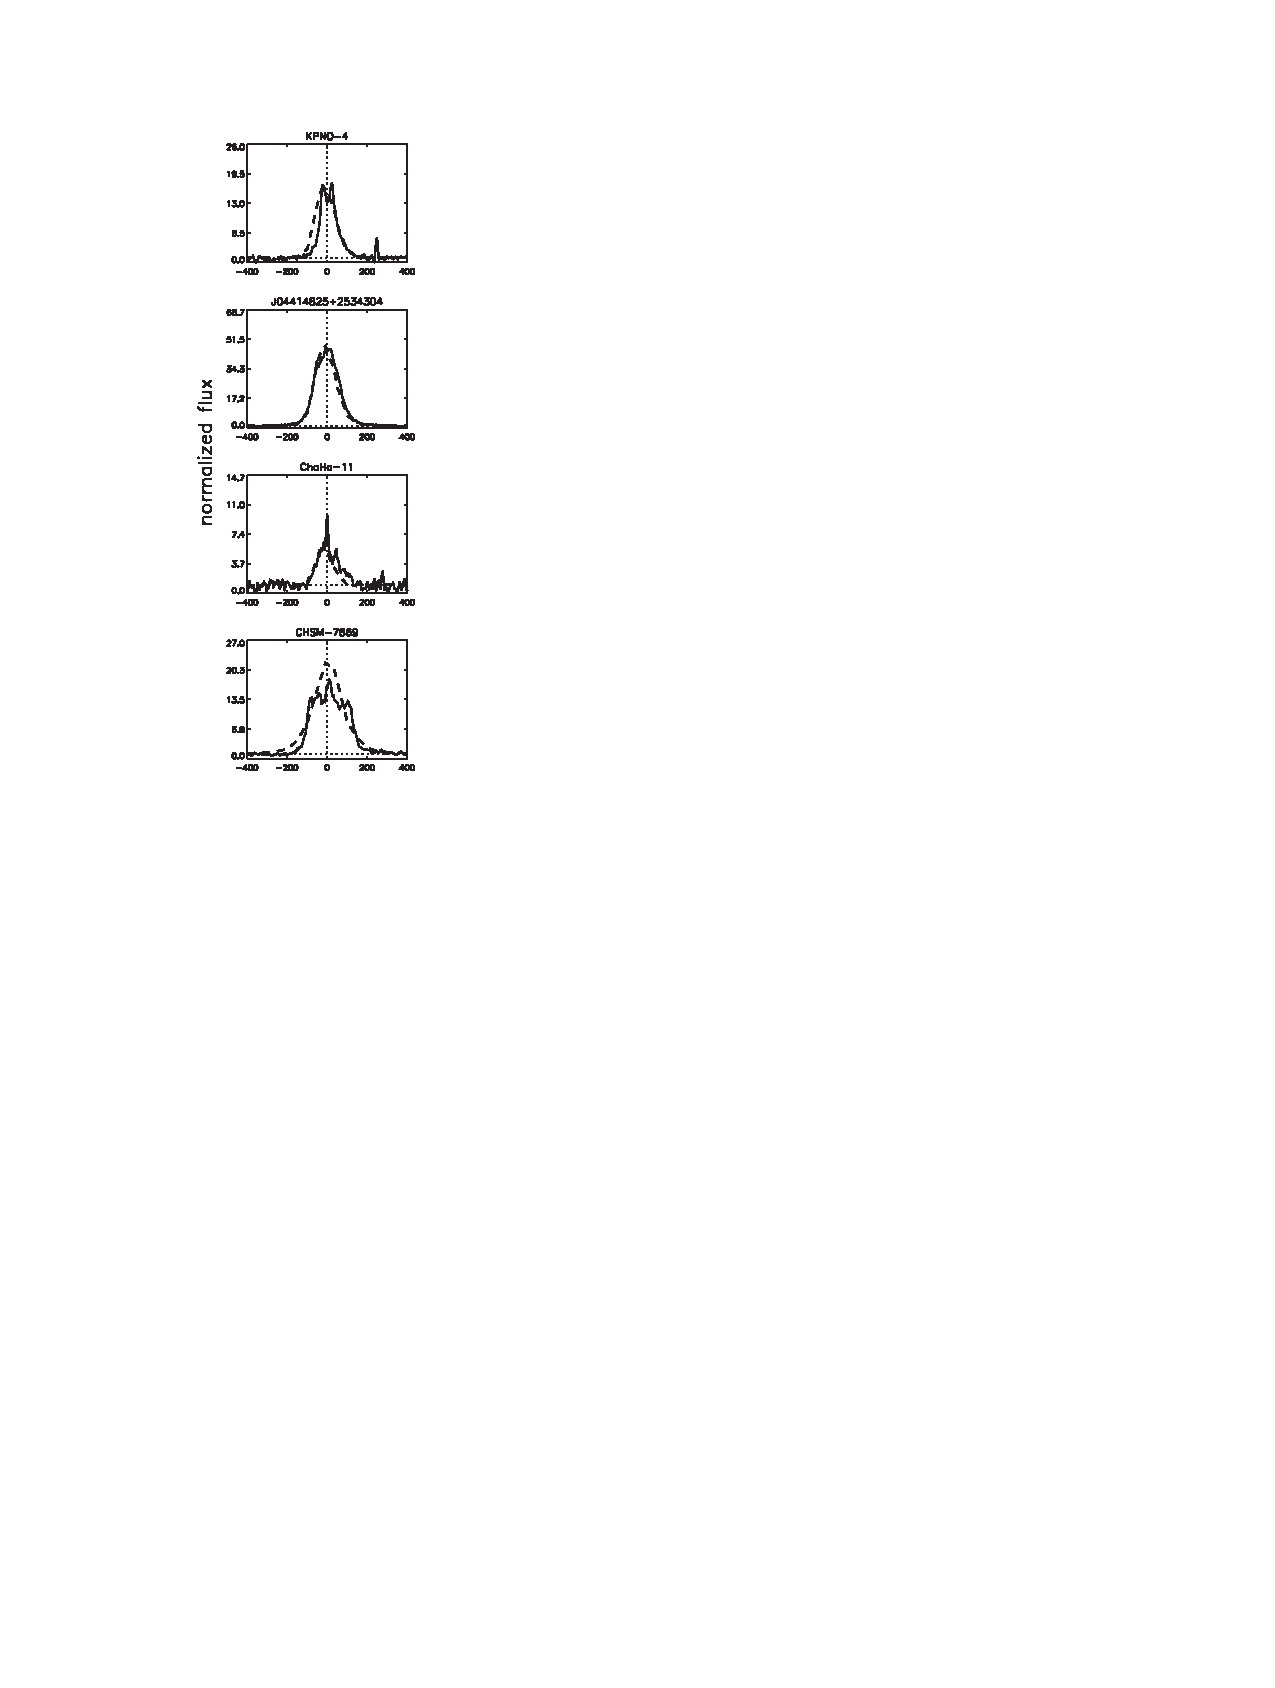
\includegraphics[width=\linewidth]{tts_ha_muzerolle05}
\caption[H$\alpha$ lines from T Tauri stars compared to models]{
\label{fig:tts_ha_muzerolle05}
Comparisons between observed (solid) and model (dashed) H$\alpha$ line profiles for a sample of T Tauri stars. The $x$ axis shows velocity in km s$^{-1}$. Each model curve is a fit in which the accretion rate is one of the free parameters. Credit: \citet{muzerolle05a}, \copyright AAS. Reproduced with permission.
}
\end{marginfigure}

These accretion rates are generally low enough so that accretion luminosity does not dominate over stellar surface emission. However, the estimated accretion rates are extremely uncertain, and the models used to make these estimates are very primitive. In general they simply assume that a uniform density slab of material arrives at the free-fall velocity, and covers some fraction of the stellar surface, and the accretion rate is inferred by determining the density of this material required to produce the observed spectral characteristics.

Despite this caveat, though, the H$\alpha$ line and other optical properties do seem to indicate that there must be some dense infalling material even around these stars that lack obvious envelopes. This in turn requires a reservoir of circumstellar material not in the form of an envelope, which is most naturally provided by a disk. Indeed, before the advent of space-based infrared observatories, optical indicators like this were the only real evidence we had for disks around T Tauri and Herbig Ae/Be stars.

\subsection{FU Orionis Outbursts}

There are many other interesting phenomena associated with these young stars, such as radio and X-ray flaring, but one in particular deserves mention both as a puzzle and a potential clue about disks. This is the FU Orionis phenomenon, named after the star FU Orionis in which it was first observed. In 1936 this star, an object in Orion, brightened by $\sim 5$ magnitudes in B band over a few months. After peaking, the luminosity began a very slow decline -- it is still much brighter today than in its pre-outburst state (Figure \ref{fig:fu_ori_herbig77}). Since then many other young stars have displayed similar behavior. When available, the spectra of these stars in the pre-outburst state generally look like ordinary T Tauri stars.

\begin{figure}
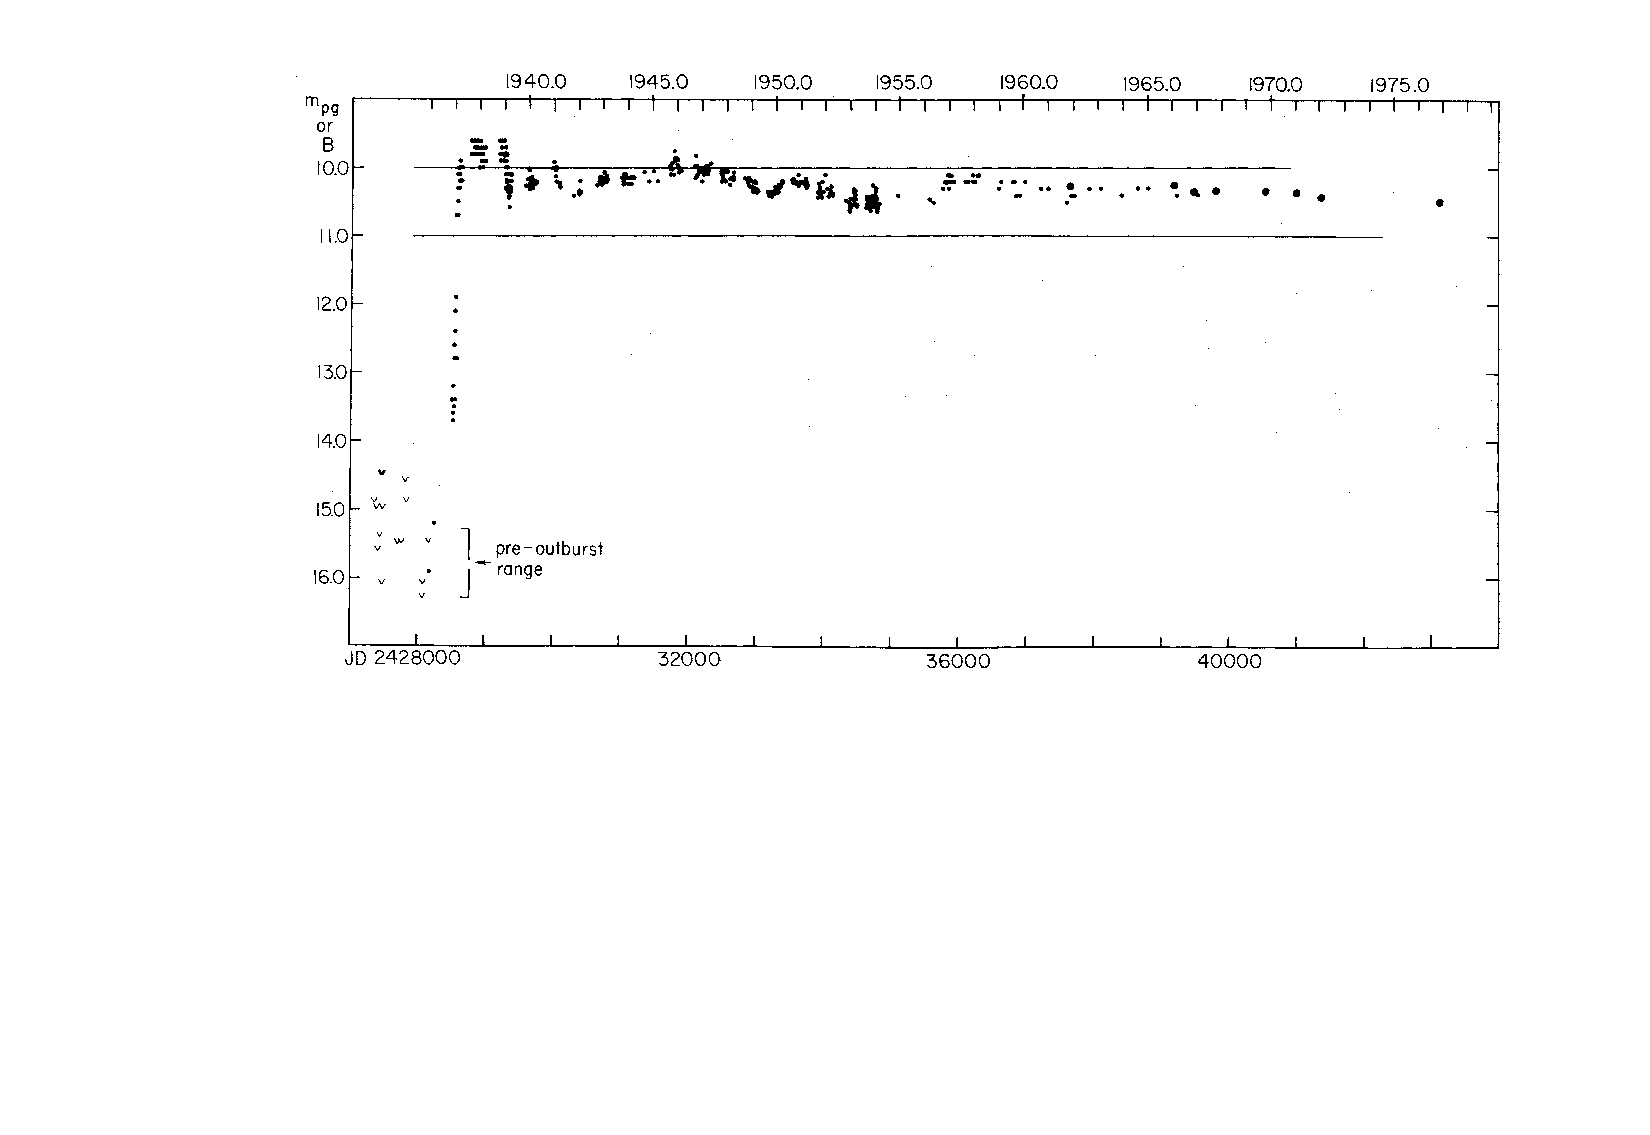
\includegraphics[width=\linewidth]{fu_ori_herbig77}
\caption[Long-term light curve of FU Orionis]{
\label{fig:fu_ori_herbig77}
A light curve of the star FU Orionis, from the 1930s to 1970s. The $y$ axis shows the apparent magnitude in B band, or from photographic observations prior to filter standardization. Credit: \citet{herbig77a}, \copyright AAS. Reproduced with permission.
}
\end{figure}

Some simple population statistics imply that this must be a periodic phenomenon. The rate of FU Ori outbursts within $\sim 1$ kpc of the Sun is roughly one per 5 years. The star formation rate in the same region is roughly 1 star per 50 years, so this implies that the mean number of FU Ori outbursts per young star is $\sim 10$.

The stellar brightening is accompanied by a rise in effective temperature, indicating the presence of hot emitting material. It is also accompanied by spectral features indicating both an outflowing wind and the presence of rapid rotation. Although a number of models have been proposed to explain exactly what is going on, and the problem is by no means solved, the most popular general idea is that outbursts like this are caused by a sudden rise in the accretion rate. For whatever reason, the disk dumps a lot of material onto the star, briefly raising the accretion rate from the tiny $10^{-8}$ $\msun$ yr$^{-1}$ typical of classical T Tauri stars up to values closer to those expected for still-embedded sources. The accreted material produces a large accretion luminosity, and the subsequent decay in the emission is associated with the cooling time of the gas that has undergone rapid infall. If this model is correct, the mystery then becomes what can set off the disk.

\section{Disk Dispersal: Observation}

We now turn to the disks that surround T Tauri and similar stars. Prior to the 2000s, we had very little direct information about such objects, since they are not visible in the optical. That changed dramatically with the launch of space-based infrared observatories, and the developed of ground-based millimeter interferometers. These new techniques made it possible to observe disks directly for the first time.

\subsection{Disk Lifetimes}

One of the most interesting properties of disks for those who are interested in planets is their lifetimes. This sets the limit on how long planets have to form in a disk before it is dispersed. In discussing disk lifetimes, it is important to be clear on how the presence or absence of a disk is to be inferred, since different techniques probe different parts and types of disks. Our discussion of disk lifetimes will therefore mirror our discussion of disk detection methods in Chapter \ref{ch:disks_obs}. In general what all these techniques have in common is that one uses some technique to survey young star clusters for disks. The clusters can be age-dated using pre-main sequence or main sequence HR diagrams, as discussed in Chapter \ref{ch:protostar_evol}. One then plots the disk fraction against age.

\begin{marginfigure}
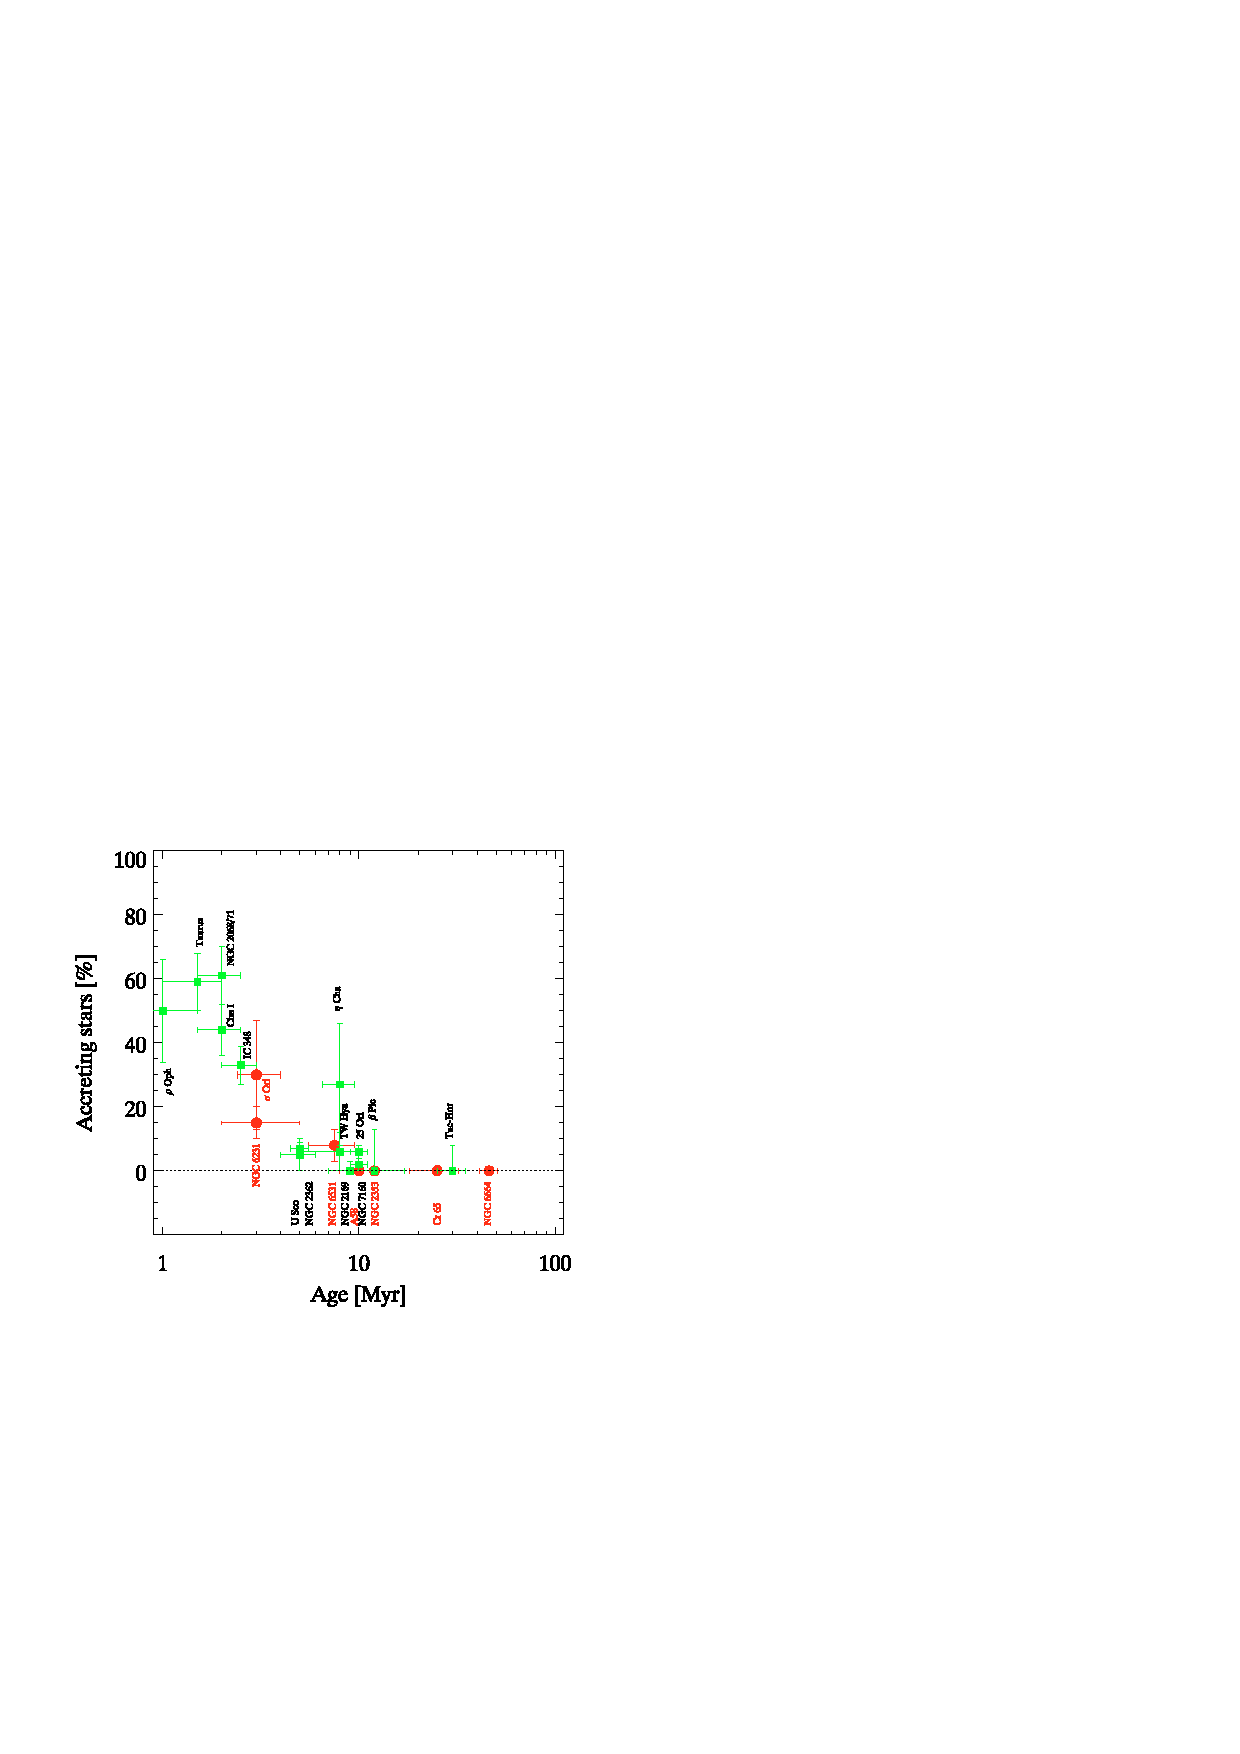
\includegraphics[width=\linewidth]{accretefrac_fedele10}
\caption[Accreting star fraction versus cluster age]{
\label{fig:accretefrac_fedele10}
Fraction of stars that show evidence of accretion, as indicated by H$\alpha$ line emission, for clusters of different ages (indicated on the $x$ axis). The names of individual clusters are marked. Credit: \citeauthor{fedele10a}, A\&A, 510, A72, 2010, reproduced with permission \copyright\, ESO.
}
\end{marginfigure}

One signature of disks we have already discussed: optical line emission associated with accretion in T Tauri stars, particularly H$\alpha$. Surveys of nearby groups find that H$\alpha$ line emission usually disappears at times between 1 and 10 Myr (Figure \ref{fig:accretefrac_fedele10}). This tells us that the inner parts of disks, $\lesssim 1$ AU, which feed stars disappear over this time scale. In contrast, ground-based near infrared observations tell us about somewhat more distant parts of the disk, out to a few AU. The timescales implied by these results are very similar those obtained from the H$\alpha$: roughly half the systems loose their disks within $\sim 3$ Myr (Figure \ref{fig:diskfrac_haisch01}).

\begin{marginfigure}
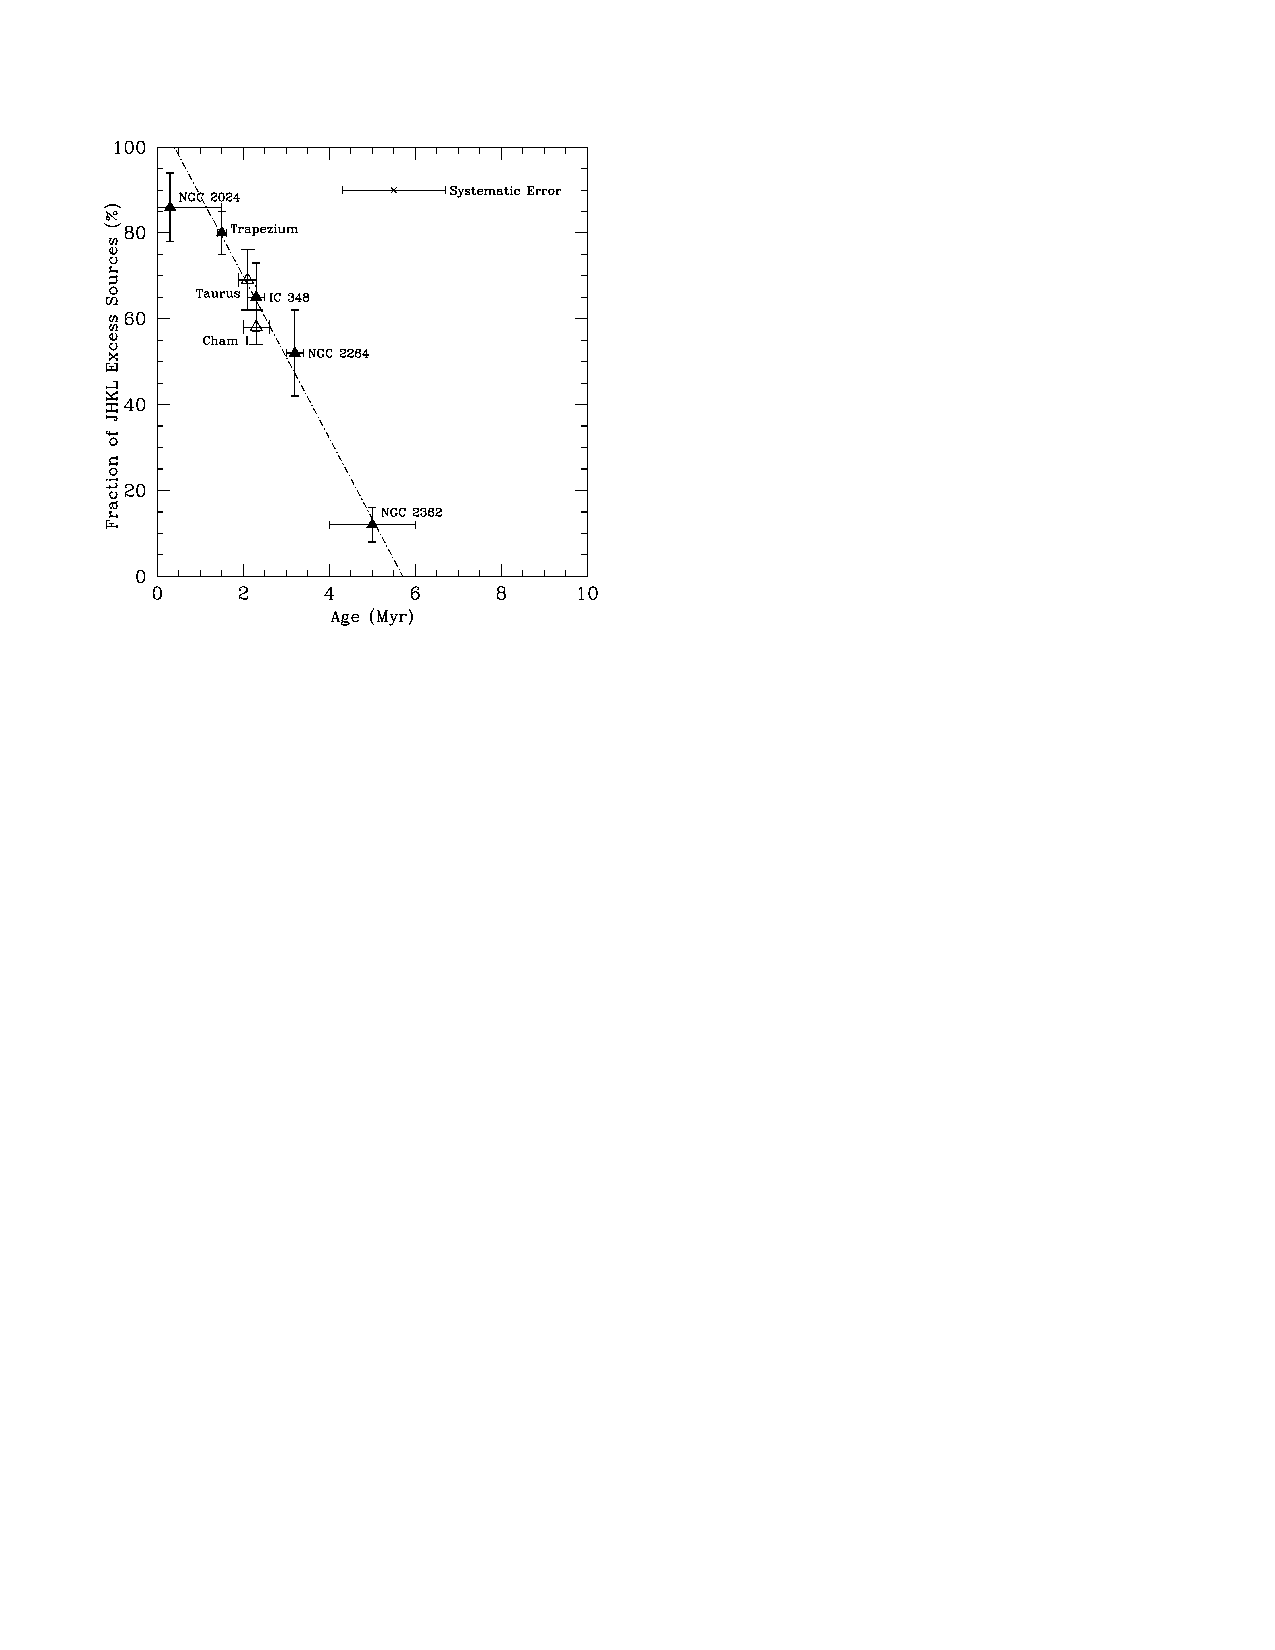
\includegraphics[width=\linewidth]{diskfrac_haisch01}
\caption[Near infrared excess fraction versus cluster age]{
\label{fig:diskfrac_haisch01}
Fraction of stars that show near-infrared excess emission versus cluster age. The names of individual clusters are marked. Credit: \citet{haisch01a}, \copyright AAS. Reproduced with permission.
}
\end{marginfigure}

These observations are sensitive primarily to the inner disk, and the infrared techniques are generally sensitive only in cases where the dust in these regions is optically thick. Some optically thin material could still be present and would not have been detected. Observations at longer wavelengths, such as \textit{Spitzer}'s 24 $\mu$m band and in the mm regime from ground-based radio telescopes, probe further out in disks, at distances of $\sim 10-100$ AU. They are also sensitive to much lower amounts of material. Interestingly, unlike the shorter wavelength observations, these measurements indicate that a small but non-zero fraction of systems retain some disks out to times of $\sim 10^8$ yr. The amounts of mass needed to explain the long wavelength excess is typically only $\sim 10^{-5}$ $M_{\oplus}$ in dust. Thus in the older systems we are likely looking at an even later evolutionary phase than T Tauri disks, one in which almost all the gas and inner disk material is gone. These are debris disks, which are thought to originate from collisions between larger bodies rather than to be made up of dust from interstellar gas.

\subsection{Transition Disks}

The observation that accreting disks and inner optically thick disks disappear on a few Myr timescales, but that some fraction leave behind very small amounts of mass in the outer disk, is a very interesting one. We will discuss theoretical models for how this happens shortly. Before doing so, however, we will review what observations tell us about the transition from gaseous, accreting T Tauri disks to low-mass debris disks.

\begin{marginfigure}
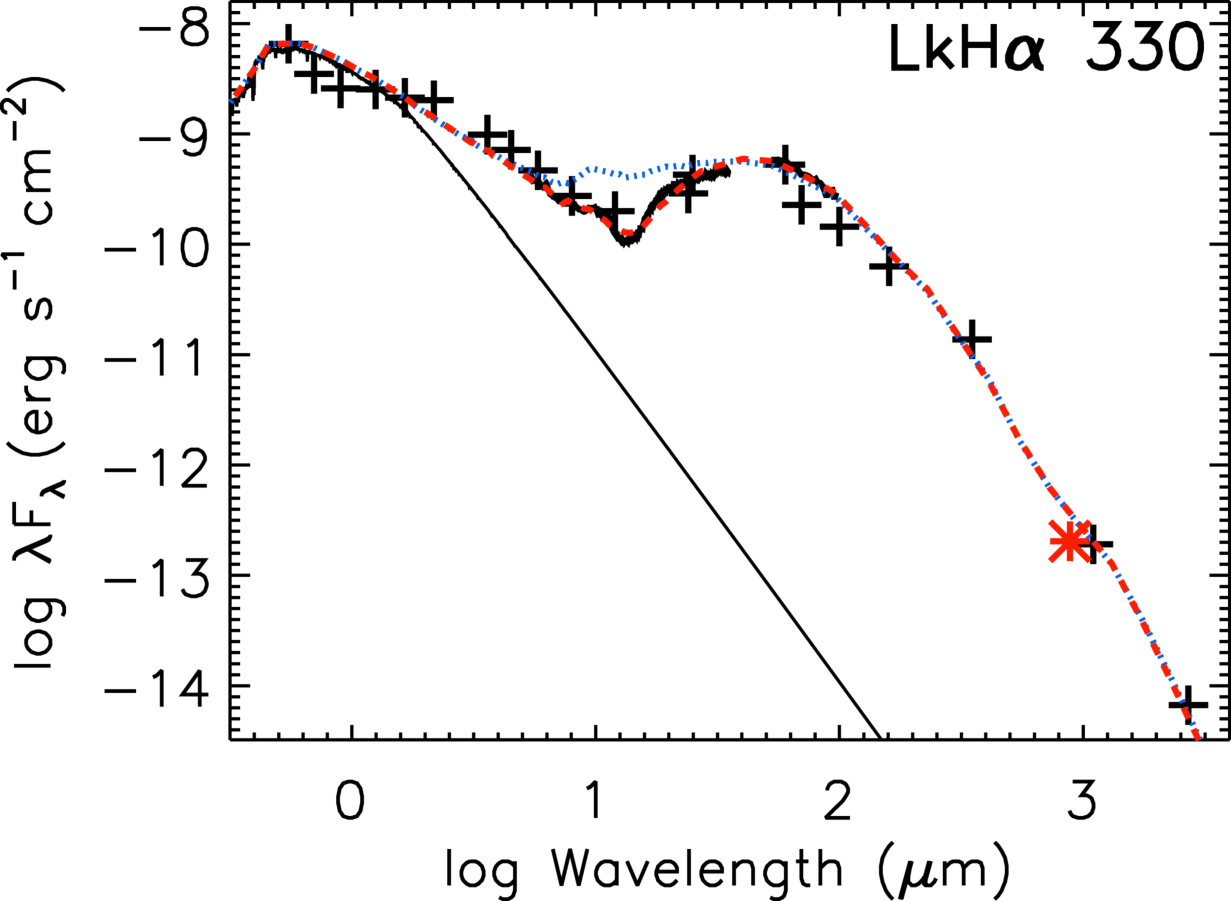
\includegraphics[width=\linewidth]{lkha330_brown08}
\caption[Spectral energy distribution of LkH$\alpha$ 330]{
\label{fig:lkha330_brown08}
The spectral energy distribution of the star LkH$\alpha$ 330. Plus signs indicate measurements. The black line is a model for a stellar photosphere. The blue line is a model for a star with a disk going all the way to the central star, while the red line is a model in for a disk with a 40 AU hole in its center. Credit: \citet{brown08a}, \copyright AAS. Reproduced with permission.
}
\end{marginfigure}

This change is likely associated with an intriguing class of objects known as transition disks. Spectrally, these are defined as objects that have a significant 24 $\mu$m excess (or excess at even longer wavelengths), but little or no excess at shorter wavelengths (Figure \ref{fig:lkha330_brown08}). This spectral energy distribution (SED) suggests a natural physical picture: a disk with a hole in its center. The short wavelength emission normally comes from near the star, and the absence of material there produces the lack of short wavelength excess. Indeed, it is possible to fit the SEDs of some stars with models with holes.

\begin{marginfigure}
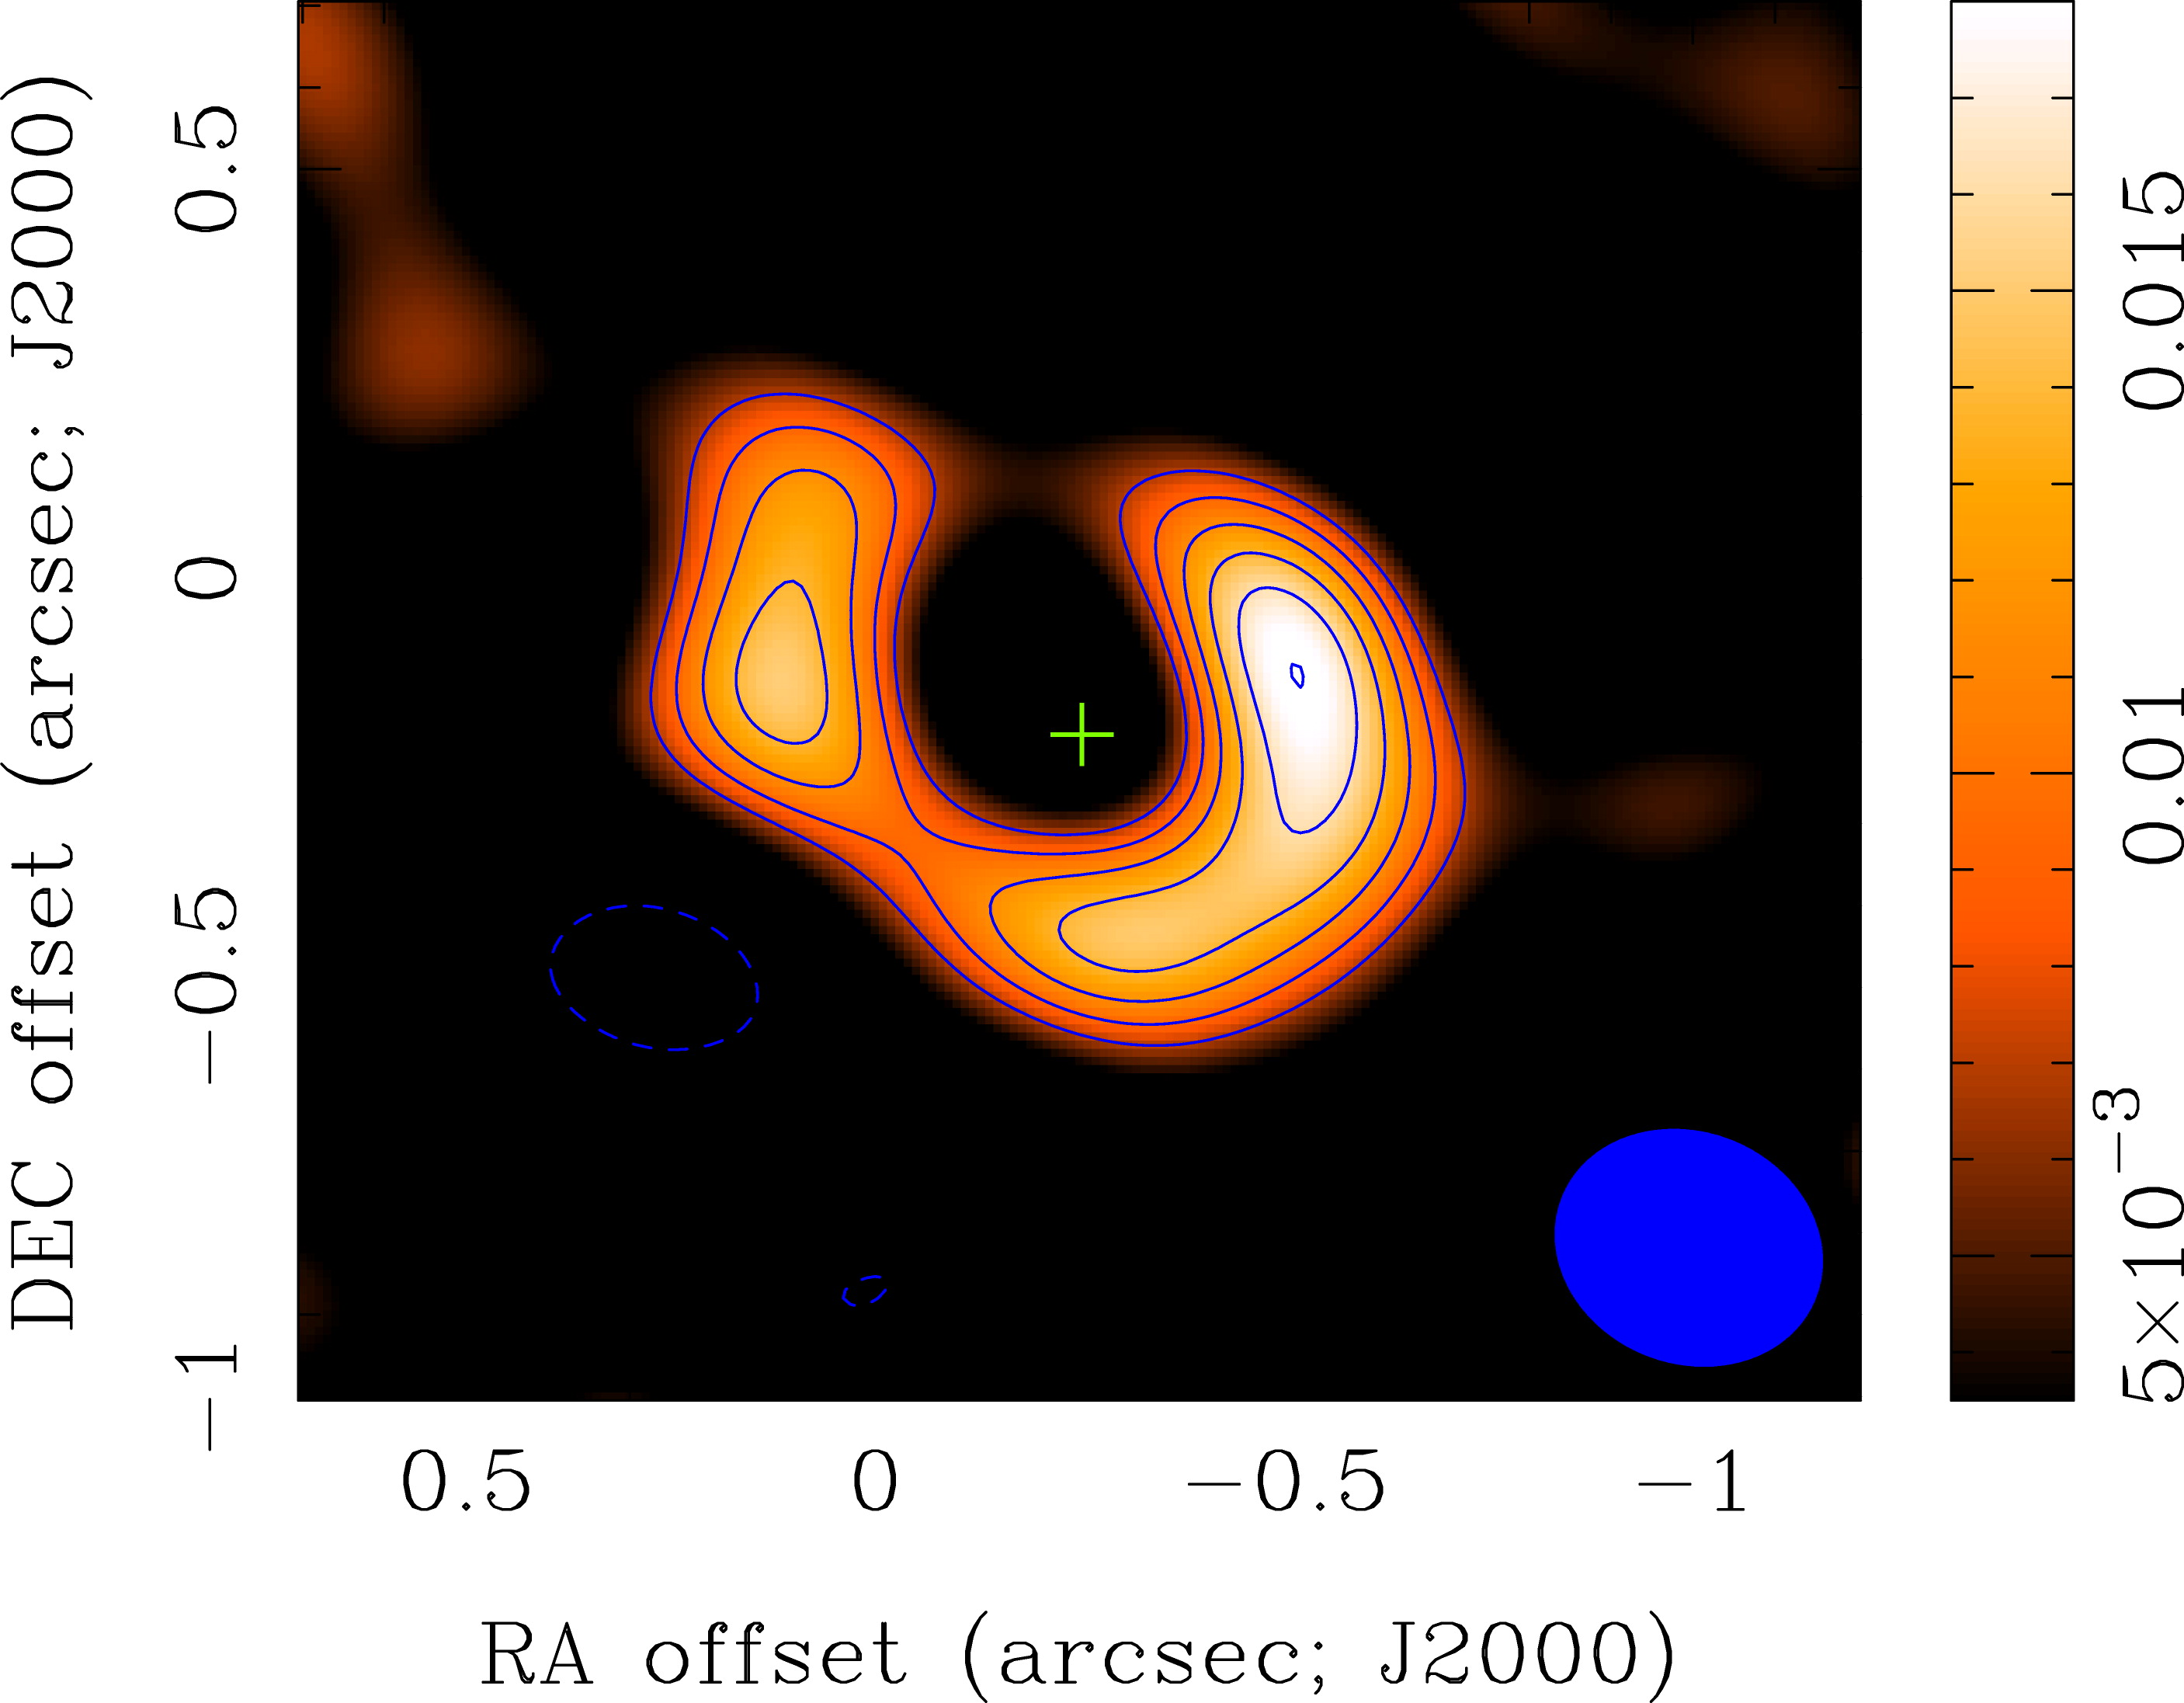
\includegraphics[width=\linewidth]{lkha330_image_brown08}
\caption[Dust continuum image of the disk around LkH$\alpha$ 330]{
\label{fig:lkha330_image_brown08}
Dust continuum image of the disk around LkH$\alpha$ 330, taken at 340 GHz by the SMA. Colors show the detected signal, and contours show the signal to noise ratio, starting from S/N of 3 and increasing by 1 thereafter. The green plus marks the location of the star. The blue circle is the SMA beam. Credit: \citet{brown08a}, \copyright AAS. Reproduced with permission.
}
\end{marginfigure}

In the last decade it has become possible to confirm the presence of inner holes in transition disks directly, at least cases where the inferred hole is sufficiently large (Figure \ref{fig:lkha330_image_brown08}). The sizes of the holes inferred by the observations are generally very good matches to the values inferred by modelling the SEDs. The holes are remarkably devoid of dust: upper limits on the masses of small dust grains within the hole are often at the level of $\sim 10^{-6}$ $M_\odot$. The sharp edges of the holes indicate that the effect driving them is not simply the growth of dust grains to larger sizes, which should produce a more gradual transition. Instead, something else is at work. However, in some transition disks, gas is still seen within the gap in molecular line emission, which also suggests that whatever mechanism is removing the dust does not necessarily get rid of all the gas as well.

\section{Disk Dispersal: Theory}

We have seen the observations suggest that disks are cleared in a few Myr. We would like to understand what mechanism is responsible for this clearing.

\subsection{Setting the Stage: the Minimum Mass Solar Nebula}

Before diving into the theoretical models, let us pause for a moment to obtain some typical numbers, which we can use below to plug in an evaluate timescales. Imagine spreading the mass in the Solar System's observed planets into an annulus that extends from each planet's present-day orbit to halfway to the next planet in each direction. Then add enough hydrogen and helium so that metal content matches that observed in the Sun. This is the mass distribution that the protoplanetary disk of the Sun must have had if all the metals in the disk wound up in planets, and if the planets were formed at their present-day locations. Neither of these assumptions is likely to be strictly true, but they are a reasonable place to begin thinking about initial conditions, and give a rough lower limit on the mass surface density of the disk from which the planets formed. We call the theoretical construct that results from this exercise the Minimum Mass Solar Nebula (MMSN). The MMSN a mass of $\sim 0.01$ $\msun$ and a surface density $\Sigma$ that varies as roughly $\varpi^{-3/2}$. The "standard" modern value for the MMSN's surface density is $\Sigma=\Sigma_0 \varpi_0^{-3/2}$, where $\Sigma_0 \approx 1700$ g cm$^{-2}$ and $\varpi_0=\varpi/\mbox{AU}$.

If solar illumination is the principal factor determining the disk temperature structure and we neglect complications like flaring of the disk, then treat the disk as a blackbody produces a temperature profile
\begin{equation}
\label{eq:TMMSN}
T=280 \varpi_0^{-1/2}\mathrm{ K}.
\end{equation}
True temperatures are probably also higher by a factor of $\sim 2$, as a result of flaring and viscous dissipation providing extra heat. The corresponding disk scale height is
\begin{equation}
H = \frac{c_g}{\Omega} = \sqrt{\frac{k_B T}{\mu m_{\rm H}}} \sqrt{\frac{\varpi^3}{GM}} = 0.03 \varpi_0^{5/4}\mbox{ AU},
\end{equation}
where $c_g$ is the gas sound speed, $\Omega$ is the angular velocity of rotation, and the numerical evaluation uses $M = M_\odot$ and $\mu=2.3$.

For solar metallicity, heavy elements will constitute roughly 2\% of the total mass, but much of this mass is in the form of volatiles that will be in the gas phase over much of the disk. For example a significant fraction of the carbon is in the form of CO and CO$_2$, and at the pressures typical of protoplanetary disks this material will not freeze out into ices until the temperature drops below $20-30$ K. Such low temperatures are found, if anywhere, in the extreme outer parts of disks. Similarly, water, which is a repository for much of the oxygen, will be vapor rather than ice at temperatures above 170 K. This temperature will be found only outside several AU.

A rough approximation to the mass in "rocks", things that are solid at any radius, and "ices", things that are solid only at comparatively low temperatures, is
\begin{eqnarray}
\Sigma_{\rm rock} & \approx & 7 \varpi_0^{-3/2}\mbox{ g cm}^{-2} \\
\Sigma_{\rm ice} & \approx &
\left\{
\begin{array}{ll}
0 & T > 170\mbox{ K}\\
23\varpi_0^{-3/2}\mbox{ g cm}^{-2} \qquad & T < 170\mbox{ K}
\end{array}
\right.
\end{eqnarray}
In other words, rocks are about $0.4\%$ of the mass, and ices, where present, are about $1.3\%$. Typical volume densities for icy material are $\sim 1$ g cm$^{-3}$, and for rocky material they are $\sim 3$ g cm$^{-3}$.

\subsection{Viscous Evolution}

Now that we have a setting, let us consider the first and most obvious mechanism for getting rid of disks: having them accrete onto their parent star. The basic process governing movement of mass in a late-stage disk is the same as during the protostellar period: viscous evolution. The difference at late stages is that there is no more mass being supplied to the disk edge, so accretion onto the star, rather than occurring in steady state, tends to drain the disk and reduce its surface density. Recall that the typical accretion rates we infer during the T Tauri phase are $\sim 10^{-9}-10^{-8}$ $\msun$ yr$^{-1}$. Since typical disk masses are $\sim 0.01$ $\msun$, this would imply that the time required to drain the disk completely into the star is $\sim 1 - 10$ Myr, not far off the observed disk dispersal lifetime.

We can make this argument more quantitative. Recall that the evolution equation for the surface density of a viscous disk is (Chapter \ref{ch:disks_theory})
\begin{equation}
\label{eq:masscons_disk_late}
\frac{\partial \Sigma}{\partial t} = \frac{3}{\varpi} \frac{\partial}{\partial \varpi} \left[\varpi^{1/2} \frac{\partial}{\partial \varpi} (\nu \Sigma \varpi^{1/2})\right],
\end{equation}
where $\nu$ is the viscosity, $\Sigma$ is the surface density, and $\varpi$ is the radius. To see how this will affect protoplanetary disks, it is useful to consider some simple cases that we can solve analytically. Let us suppose that the viscosity follows a powerlaw form $\nu=\nu_1 (\varpi/\varpi_1)^\gamma$. The equations in this case admit a similarity solution; the case $\gamma=1$ is included in problem set 4. For arbitrary $\gamma$, it is easy to verity that equation (\ref{eq:masscons_disk_late}) has the solution
\begin{equation}
\Sigma = \frac{C}{3\pi\nu_1 x^\gamma} T^{-(5-2\gamma)/(4-2\gamma)} \exp\left(-\frac{x^{2-\gamma}}{T}\right),
\end{equation}
where $C$ is a constant with units of mass over time that determines the total mass in the disk and the accretion rate, $x=\varpi/\varpi_1$, and $T$ is a dimensionless time defined by
\begin{equation}
T = \frac{t}{t_s}+1
\qquad
t_s = \frac{1}{3(2-\gamma)} \frac{\varpi_1^2}{\nu_1}.
\end{equation}
In this similarity solution, at any given time the disk surface density has two regions. For $x^{2-\gamma} \ll T$, the exponential term is negligible, and the surface density simply follows a powerlaw profile $x^{-\gamma}$. For $x^{2-\gamma} \gg T$, the exponential term imposes an exponential cutoff. As time goes on and $T$ increases, the powerlaw region expands, but its surface density also declines (at least for $\gamma < 2$, which is what most physically-motivated models produce). The quantity $t_s$ is the characteristic viscous evolution time. For times $t\ll t_s$, $T$ is about constant, so there is no evolution. Evolution becomes significant after $t>t_s$.

If we adopt a simple $\alpha$ model with constant $\alpha$, then recall that $\nu = \alpha c_g H$. For our MMSN, $T \approx 280 \varpi_0^{-1/2}$ K and $H \approx 0.03 \varpi_0^{5/4}$ K. Since $c_g\propto T^{1/2}$, this implies $\nu\propto \varpi$:
\begin{equation}
\nu \approx 5\times 10^{16} \alpha \varpi_0\mbox{ cm}^2\mbox{ s}^{-1}.
\end{equation}
Thus constant $\alpha$ for our MMSN corresponds to $\gamma = 1$. Plugging this value into the similarity solution gives $t_s = 0.024\alpha_{-2}^{-1}\mbox{ Myr}$, where $\alpha_{-2} = \alpha/0.01$. Thus we would expect the disk to drain into the star in $\sim 1$ Myr if it had values of $\alpha$ expected for the MRI.

This might seem like an appealing explanation for why disks disappear, but it faces two serious objections. The first is that, as discussed in chapter \ref{ch:disks_theory}, magnetorotational instability (MRI) seems unlikely to be able to operate everywhere in the late-stage disks. The surface will be kept ionized by stellar radiation and possibly cosmic rays, but the midplane will be too neutral for strong magnetic coupling. This should reduce the accretion rate.

A second, more serious objection is that it does not reproduce the observation that disks drain inside-out (or at least some of them do). In this model, the surface density everywhere inside the powerlaw inner region decreases with time as $t^{-3/2}$, meaning that the disk would fade uniformly rather than from the inside out. While this result is for the particular similarity solution we used, it is a generic statement that, in any model where $\alpha$ is constant with radius, the disk will tend to drain uniformly rather than inside-out. Thus something more sophisticated is needed.


\subsection{Photoevaporation Models}

One mechanism that has been proposed for disk clearing is photoevaporative winds. We will not discuss this quantitatively here, because a basic model of this process is left as an exercise in Problem Set 5. The qualitative picture is simply that the surface of the disk is heated to temperatures of $\sim 100-200$ K by stellar FUV radiation out to a fairly large region, and is heated to $\sim 10^4$ K by ionizing radiation closer in to the star. If the heated gas is far enough from the star for this temperature increase to raise its sound speed above the escape speed, it will flow away from the disk in a thermally-driven wind.

This tends to produce maximum mass loss from a region near where the sound speed equals the escape speed, since that is where there is the most gas and the radiation is most intense, but the gas can still escape. If the radiation is intense enough, a gap in the disk will open at this radius, and mass will not be able to pass through it -- any gas that gets to the gap is lost in the wind. As a result the inner disk drains viscously, and is not replenished, leaving a hole like we observe.

\subsection{Rim Accretion Models}

A second mechanism that could produce an inner hole is rim accretion. In this picture, MRI operates only on the inner rim of the disk where the gas is exposed to direct stellar radiation. Material from this rim accretes inward while the rest of the disk remains static. As the rim accretes, more disk material is exposed to stellar radiation and the MRI-active region grows. Thus the disk drains inside-out. Our treatment of this phenomenon will generally follow that set out by \citet{chiang07a}.

In this picture, we let $N_*$ be the column (in H atoms per cm$^2$) of material in the rim that is sufficiently ionized for MRI to operate. In this case the mass in the MRI-active rim at any time is
\begin{equation}
M_{\rm rim} = 4\pi N_* \mu_{\rm H} r_{\rm rim} H,
\end{equation}
where $r_{\rm rim}$ is the rim radius, $H$ is the scale height at the rim, and $\mu_{\rm H}$ is the mass per H nucleus. The time required for this material to accrete is the usual value for viscous accretion:
\begin{equation}
t_{\rm acc} = \frac{r_{\rm rim}^2}{\nu} = \frac{r_{\rm rim}^2}{\alpha c_g H},
\end{equation}
where $c_g$ is the gas sound speed in the irradiated rim, which is presumably higher than in the shielded disk interior. Putting these together, we expect an accretion rate $\sim M_{\rm rim}/t_{\rm acc}$. \citet{chiang07a}, solving the problem a bit more exactly, get
\begin{equation}
\dot{M} \approx \frac{12 \pi N_* \mu_{\rm H} \alpha c_g^3 r_{\rm rim}^2}{G M}.
\end{equation}
One can estimate $N_*$ and $c_g$ from the thermal and ionization balance of the irradiated rim, and \citet{chiang07a}'s result is $N_* \approx 5\times 10^{23}$ cm$^{-2}$ and $c_g \approx 0.9$ km s$^{-1}$, giving
\begin{equation}
\dot{M} = 1.4\times 10^{-11} \alpha_{-2} M_0^{-1} r_{\rm rim,0}^{2} \,\msun\mbox{ yr}^{-1},
\end{equation} 
where $M_0$ is the stellar mass in units of $\msun$ and $r_{\rm rim}$ is the rim radius in units of AU.

This model nicely explains why disks will drain inside out. Moreover, it produces the additional result that any grains left in the disk that reach the rim will not accrete, and are instead blown out by stellar radiation pressure. This produces an inner hole with a small amount of gas on its way in to the star, as is required to explain the molecular observations, but with no dust.

\subsection{Grain Growth and Planet Clearing Models}

The final possible mechanism for getting rid of the disk is the formation of planets. If the dust in a disk agglomerates to form larger bodies, then the opacity per unit mass will drop dramatically, and as a result the disk will cease to produce observable infrared or millimeter emission. If the planetesimals further agglomerate into planets with significant gravitational effects, these can begin to clear the gas as well. We will therefore end this chapter with a discussion of how grains might begin to agglomerate together, starting the process of getting rid of a disk by planet formation that will be the subject of Chapter \ref{ch:planets}.

Consider a population of solid particles radius $s$, each of which individually has density $\rho_s$. The number density of particles (i.e., the number of particles per cm$^{3}$) is $n$, so the total mass density of the population of solids is
\begin{equation}
\rho_d = \frac{4}{3}\pi \rho_s s^3 n
\end{equation}
If the collection of solids has a velocity dispersion $c_s$, the mean time between collisions between them is
\begin{equation}
t_{\rm coll} = (n \pi s^2 c_s)^{-1} = \frac{4}{3} \frac{\rho_s s}{\rho_d c_s}
\end{equation}
We will see in a little while that grains of interstellar sizes will have about the same scale height as the gas. Thus, within one scale height of the disk midplane, we may take 
\begin{equation}
\rho_d \approx \frac{\Sigma_d}{H} = \frac{\Sigma_d \Omega}{c_g},
\end{equation}
where $\Sigma_d = \Sigma_{\rm rock} + \Sigma_{\rm ice}$ is the total surface density of "dust", including both rocky and icy components. 

The velocity dispersion of the solids $c_s$ depends on their sizes. In the case of small grains it will simply be the typical velocity imparted by Brownian motion in the fluid, which is
\begin{equation}
c_s = \sqrt{\frac{3}{2} \frac{k_B T}{m_s}} = \sqrt{\frac{3 \mu m_{\rm H}}{2 m_s}} c_g \approx 0.1 \varpi_0^{-1/4} s_{-4}^{-3/2} \rho_{s,0}^{-1/2}\mbox{ cm s}^{-1}
\end{equation}
where $m_s = (4/3)\pi s^3 \rho_s$ is the mass of the solid particle, $\rho_{s,0}=\rho_s/(1\mbox{ g cm}^{-3})$, $s_{-4} = s/(1\,\mu\mbox{m})$, and we have used our fiducial MMSN to estimate $c_g$. Plugging $n$ and $c_s$ into the collision time, we have
\begin{eqnarray}
t_{\rm coll} & \approx & \frac{4\sqrt{2}}{3\sqrt{3}}\frac{s\rho_s}{\Sigma_d \Omega}\sqrt{\frac{m_s}{\mu m_{\rm H}}} = \frac{8\sqrt{2\pi}}{9} \sqrt{\frac{\rho_s^3 s^5}{\Sigma_d^2\Omega^2 \mu m_{\rm H}}}
\nonumber \\
& = & (2.6, 0.6) \varpi_0^3 \rho_{s,0}^{3/2} s_{-4}^{5/2}\mbox{ yr},
\end{eqnarray}
where the two coefficients refer to the cases of rock only, or rock plus ice.

The bottom line of this calculation is that the small particles that are inherited from the parent molecular cloud will very rapidly collide with one another in the disk: a 1 $\mu$m-sized particle can expect to run into another one roughly 1 million times over the $\sim 1$ Myr lifetime of the disk. As the particles grow in size, collisions will rapidly become much less rapid, and will reach one collision per Myr at around 0.25 mm. Of course this assumes that the particles remain distributed with the same scale height as the gas, which is not a good assumption for larger particles, as we will see.

Before moving on, though, we must consider what happens when the particles collide. This is a complicated question, which is experimentally difficult enough that some groups have constructed dust-launching crossbows to shoot dust particles at one another in an attempt to answer experimentally. For very small particles, those of micron sizes, the answer is fairly easy. Such particles will be attracted to one another by van der Waals forces, and when they collide they will dissipate energy via elastic deformation. Theoretical models and experiments indicate that two particles will stick when they collide if the collision velocity is below a critical value, and will bounce or shatter if the velocity is above that value.

For 1 $\mu$m particles, estimated sticking velocities are $\sim 1-100$ cm s$^{-1}$, depending on the composition of the body, and that this declines as $\sim s^{-1/2}$. Since this is much more than the Brownian speed, $1-10$ $\mu$m particles will very quickly grow to large sizes. Thus we have a strong theoretical prediction that grains should grow in disks. We will return to the question of how far this growth goes in the next chapter.


